\chapter{Testing Usability and Effectiveness on a Wider Audience}
\label{chap:userstudy}

Our evaluation of CrashSimulator has shown that it is able to find new environmental bugs in widely deployed software. Following this success, we wanted to see if it
could be effective when employed by outside developers.
After all, it's initial ``users'' in the study were developers with a high degree of expertise in its operation.

To investigate the usability of the tool,
we designed and conducted a study in which 12 undergraduate and graduate students with varying levels of experience went looking for bugs in commonly used applications.
The study took place over the course of six sessions
of a special topics Systems Security class (CSGY-9963) in the fall of 2019.
Each class began with 20
minutes of instruction on aspects of using the tool, followed by 70 minutes of active investigation. Participants employed
CrashSimulator to find bugs, and then constructed patches to fix
them.
They were asked to record their progress
using a provided work log template in which participants documented
how they went about using CrashSimulator. 
Each weekly entry listed what application the participant was
investigating,  what bugs they found, and any interesting details discovered along the way. An example of such a log may be found in Figure~\ref{fig:examplereport}.
It should be noted that this study was conducted {\tt before} the work on PORT discussed in Chapter~\ref{chap:port}.
As such,
PORT was not available for use by our participants.

Our goal for this user study was two-fold.  First and foremost,
we wanted to see if the participants were able to use CrashSimulator to find bugs with no previous experience and only limited instruction.
We discuss these results in~\ref{subsec:bugs-by-participants}, and summarize the bugs that were found.
Second, we wanted the participants to help us identify usability issues
or flaws within the tool itself. These observations are shared in~\ref{subsec:crashsim-patches}. Finally, we share our observations
of how participants interacted with the tool, and what shortcomings
it revealed in~\ref{subsec:tool-shortcomings}.

\section{Study Parameters}
\label{sec:studyparameters}

Though the design of this study is fairly basic, a few details on how it was conducted are called for. As stated above, all participants were students enrolled in an Application Security class.
All participants worked independently during class time, though they had the option to ask for assistance from one of CrashSimulator's developers should they encounter problems with the tool.
They were also encouraged to work on this effort on their own time outside of class.
Second, we allowed participants to select which applications they would test.
In general, they gravitated towards widely deployed, simple, command line applications.
This is likely because these sorts of applications require much less initial setup.

It is important to note that all tables and bug counts reported in earlier
chapters do not reflect the results discussed in this chapter.
We decided to count evaluation bugs and user study bugs separately because two of the bugs found in the user study
had been previously identified
in our evaluation.
The overlapping bugs were found independently,
as the participants weren't aware of the paper or the evaluation results.
We enforced this separation to ensure our total counts were not inflated.
Finally, this study was reviewed and categorized as ``exempt'' by NYU's Institutional review board.
We received this designation in part because we made the decision not to capture any demographic information. Given that the goal of our study was to measure the usability of the tool, we deemed it not necessarily to solicit the more personal data that would mandate a more detailed review by the IRB.

\newgeometry{left=2cm}
\begin{figure}[btp]
\centering
\fbox{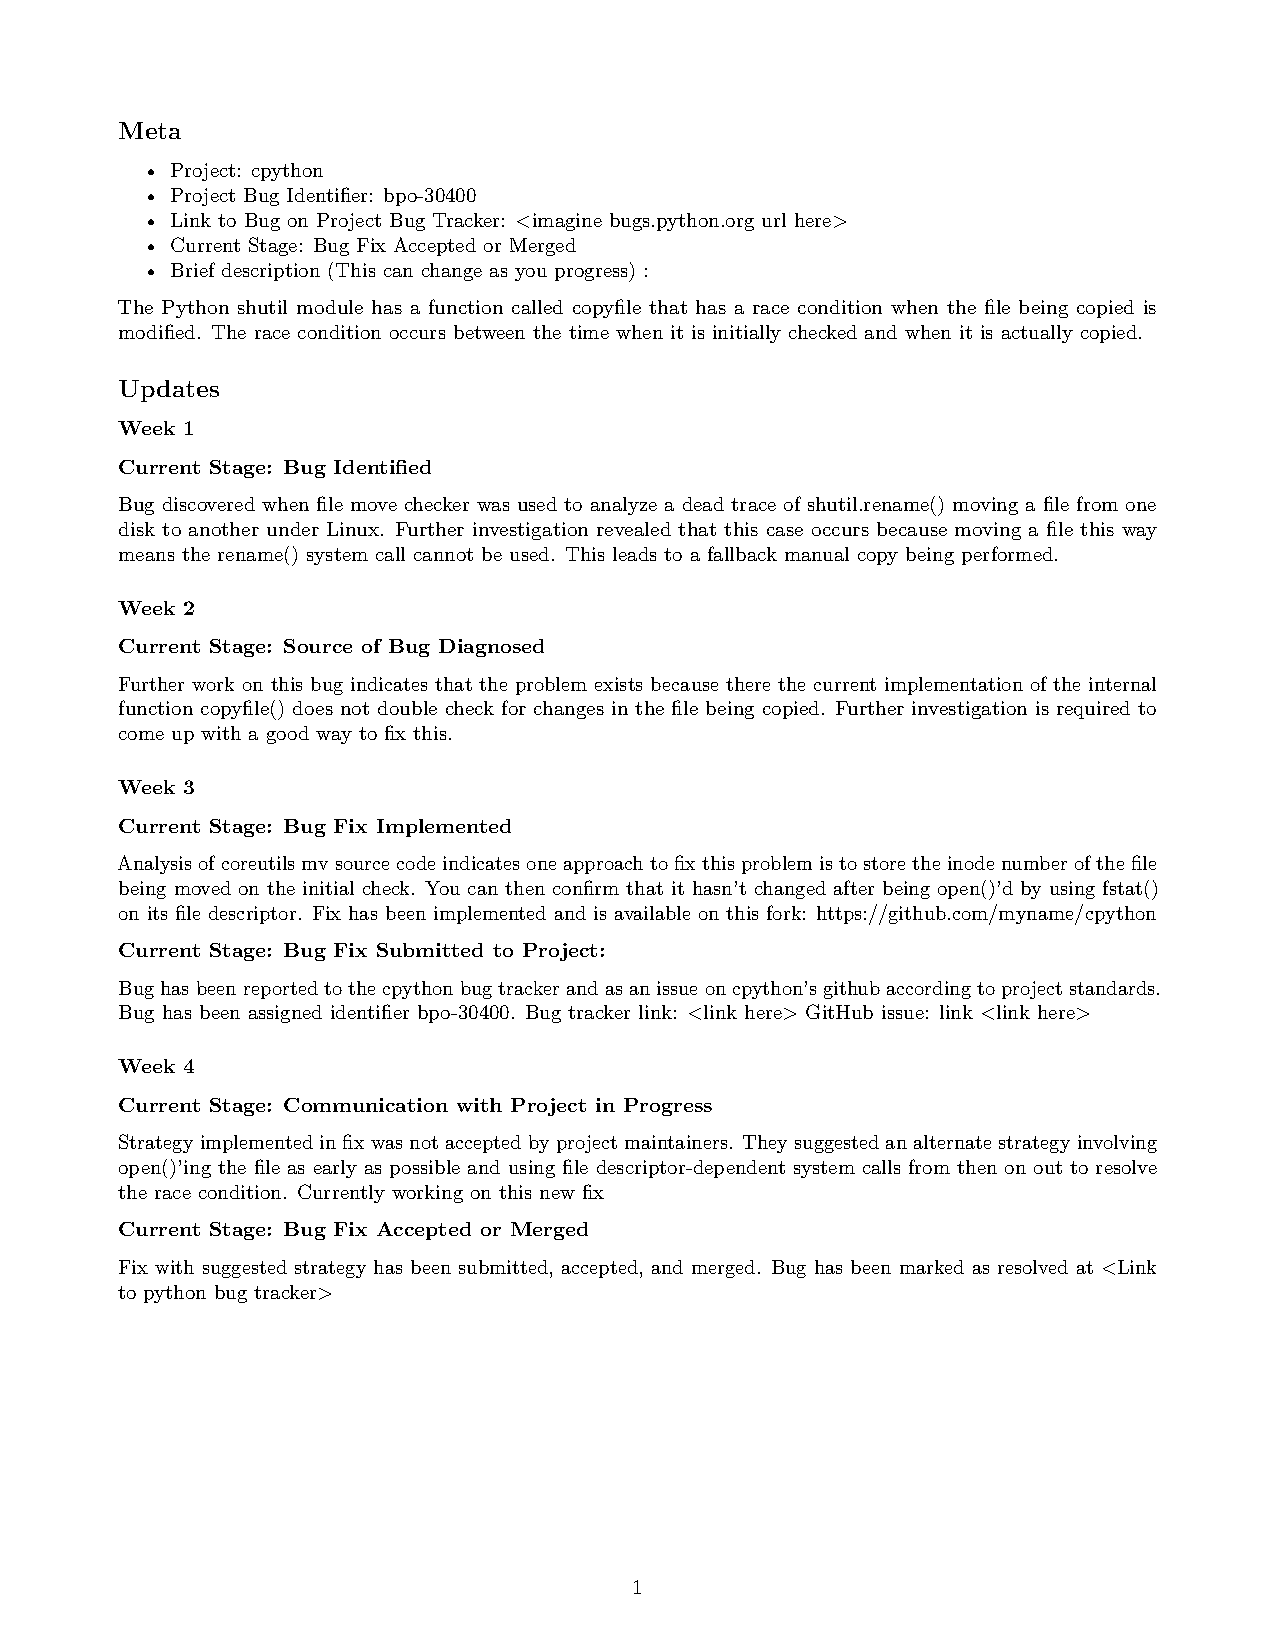
\includegraphics[scale=.8]{chapter5/figures/examplereport}}
\caption[Example Progress Report]{Example Progress Report}
\label{fig:examplereport}
\end{figure}
\restoregeometry

\section{Results: Bugs Found by Participants}
\label{subsec:bugs-by-participants}
Study participants found a total of 18 bugs using CrashSimulator's
``Unusual Filetype Mutator.''
Participants constructed patches to correct six of these bugs and submitted
them to the appropriate maintainers.
An example of one such patch is listed in Figure~\ref{fig:participantpatch}.

Although some of our participants were able to diagnose and fix the bugs they found,
none of their submitted patches were accepted.
There are several specific reasons why this happened:

\paragraph{Patches Submitted to the Wrong Maintainer}
The most common reason for rejection was some participants submitted their patch to the wrong maintainer.
Most were submitted to Ubuntu Linux's main bug tracker, which is intended to manage distribution-specific bugs.
In these cases,
maintainers classified the bugs as ``WONTFIX'' and referred the submitter to the correct upstream project.
This response indicates that our participants were unaware of the relationship between distribution maintainers and application maintainers.
This deficiency makes it clear that further instruction is needed about the importance of sending patches to the correct place.

\paragraph{Overly Broad Patches}
A second reason that patches were rejected is because they were considered ``overly broad'' by the maintainers that reviewed them.
An example of this case is a patch for ``sort,'' which would disallow it's processing of anything but regular files.
This would break a very common usage of the tool in which a user ``pipes'' in the output of another utility.
Situations like this suggest that the writer did not fully grasp the implications of the patch they constructed.
Typically this is resolved through dialog between the submitter and maintainer with the goal of producing a mutually acceptable patch.
In this specific case, the participant did not follow up further with the maintainer.

\paragraph{``Not A Bug''}
A final common outcome was that patches were rejected because the behavior they intended to fix was deemed ``not a bug'' by the receiving maintainer.
This opinion stems from varying definitions of ''application misbehavior.''
In our work on the SEA technique and CrashSimulator, we argued that  consuming large amounts of resources or running forever constituted undesirable behavior in an application.
The maintainer in this case argued that such outcomes may be correct
for some usages.
This is another situation where discussions between the submitter and maintainer would be needed to derive an acceptable fix.

Even though the generated patches were not accepted,
the results remain
important as a confirmation that 
users other than the original development team
can find bugs in real world applications with our tool.
Participants commented that narrowing the source of a bug
down to a particular sequence of system calls
was helpful in itself. Identifying the area of
code responsible for the bug decreased the time required to produce a fix.
Though observations of study participants
confirmed that familiarity with operating systems concepts
made it easier to work with CrashSimulator, even
those without this background were able to identify bugs using the
built-in anomalies.


 \begin{figure}
 \begin{lstlisting}[basicstyle=\ttfamily,gobble=4]
     --- ./coreutils_original/coreutils-8.28/src/uniq.c
     +++ ./src/uniq.c
     @@ -333,6 +333,11 @@
      {
        struct linebuffer lb1, lb2;
        struct linebuffer *thisline, *prevline;
     +  struct stat sb;
     +
     +  stat(infile, &sb);
     +  if (S_ISBLK (sb.st_mode) || S_ISCHR (sb.st_mode))
     +    die (EXIT_FAILURE, errno, "error opening device file %s",
              quotef (infile));

        if (! (STREQ (infile, "-") || freopen (infile, "r", stdin)))
          die (EXIT_FAILURE, errno, "%s", quotef (infile));
\end{lstlisting}
\caption[Participant Submitted Patch]{Example of a patch submitted by a CrashSimulator user study participant.
This patch prevents the coreutils `uniq` utility from processing block devices. }
\label{fig:participantpatch}
\end{figure}

\section{Results: Tool Limitations Identified by Participants}
\label{subsec:crashsim-patches}

One of the benefits of open source software is that it can be maintained and improved by its user community.
This user study indicates that CrashSimulator is capable of garnering this sort of interaction from its users.
Students submitted five patches
to the tool's code over the
course of the study period.
Three of these reports included patches built by the reporting students that directly
corrected a bug.
The remaining patches fixed issues with the scripts responsible for installing CrashSimulator.

The students also submitted 16 reports identifying unsupported system calls, and reported 17 bugs in
existing system call handlers or test orchestration code.
On the one hand, these results are encouraging.  The necessity of adding
support for new system calls
indicates that the students were
using CrashSimulator to test a wide variety of new applications.
On the other hand, the number of bug reports not related to system call support
indicates there is still work to be done on the tool.


\section{Instructor Observations}
\label{subsec:tool-shortcomings}
Observations of how students worked  with the tool during the study were also revealing.
First,
it became clear that the tool
lacks a dedicated mechanism
for determining
which application behaviors constitute a ``bug.''
For example, an application's developer
may have intended that an application processing an ``infinitely long'' file should run continuously
until killed by an outside command.
Therefore, that behavior should not be classified as a bug.
Second,
it demonstrated that
simply reporting if an application did or did not change its behavior
in the presence of an anomaly may not provide sufficient data to identify a bug. The specific results that indicate the presence of a bug must be made clearer to the user.
Both of these issues could be corrected 
by improving the tool's output.
Clearer descriptions of a given result
can give a better idea of
if,
and why,
users should be concerned.

To conclude, our user study has revealed both strengths and weakness
of the CrashSimulator tool.
We were encouraged by the fact that participants were able to find bugs in and build patches for real world applications.
Thus, we feel our results show CrashSimulator is usable by outside developers even if there is still work to be done in getting these patches accepted. 
We are also pleased with the improvements that came to the tool as a result of the collaboration between study participants and CrashSimulator's developers.
The tool has had numerous bug fixes and usability enhancements as a result of this effort.
We hope that such collaboration will be a cornerstone of the CrashSimulator project as we push for its wider adoption.

\section{Open Source Bug Reporting}

In light of the above, it is worth briefly discussing correct procedures for reporting bugs in open source projects and how this may have affected our ability to get patches adopted. It's important to remember that by the time an application makes it to a user's computer via a package manager, it has been handled by numerous different parties. So, deciding who should receive patches will be dictated by the type of bug and where it was found. 

First, the preferred contact point for application bugs would be  
the project's primary developers, as these are the individuals who build and maintain the application itself.
A second point of contact might be the distribution developers who may apply distribution-specific patches. For example, Debian maintains and applies a patch to its locale-related tools so locale configuration changes will be automatically picked up and applied.
These developers are the best point of contact for bugs and fixes related to these distribution-specific functions.

Finally,
there are the maintainers that deal with 
packaging and distributing the application.
These developers assemble an installable package from the artifacts produced by upstream efforts.
In the process they often make installation and configuration decisions in order to give end users a smoother experience. 
Therefore, concerns related to packaging and installation would be handled by these maintainers.
Given that many of our patches were submitted to incorrect maintainers,
explicitly explaining this process to our participants would have likely lead to more success.

Based on the above division of concerns,
it is evident that submitting bugs or fixes to the proper maintainers is of paramount importance.
Our results point to a definite gap in how students are taught about working with open source projects.
Instructors need to spend at least a  small amount of time explaining how these projects are organized.
Submitting patches to the appropriate maintainer on the first attempt would have saved the turn around time necessary for distribution maintainers to triage the patch and recommend it be submitted upstream.
This savings may have allowed the patches to be accepted within the study's allotted time.